\label{sec:VOT}
% \paragraph{VOT in the onset}
\begin{figure}
 \centering
 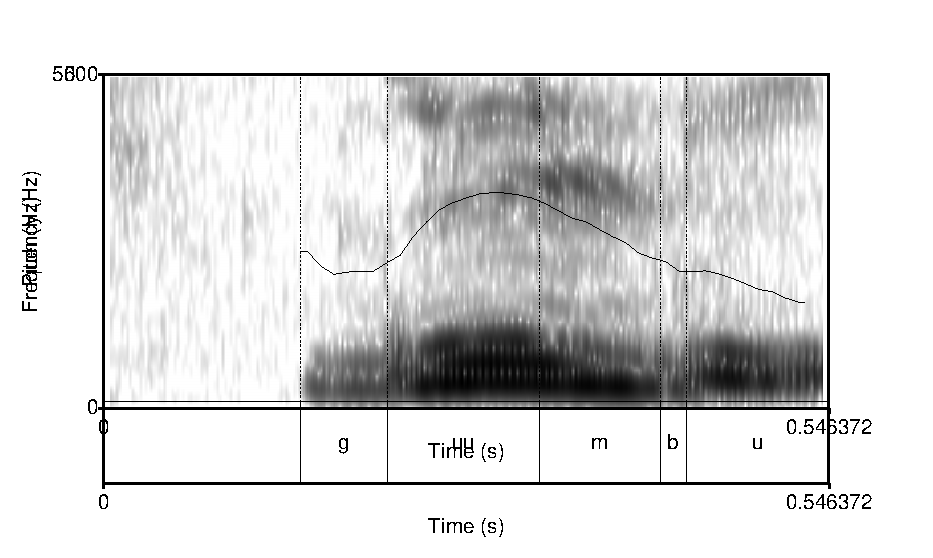
\includegraphics[height=0.3\textheight]{./pics/guumbu-a.eps}

 \includegraphics[height=0.3\textheight]{./pics/inithumpathpadayam.eps}

 \caption{[g] in the absolute onset of \phontrs{gu:\umb u}{Negombo (town)} is fully voiced and has a negative VOT of about 0.068s (above). This can be seen from the pitch contour, which is present during the whole articulation of g. Since pitch can only be measured on voiced parts, the pitch contour can be used to identify voicing. The image below shows that the pitch contour is absent for  [\dentt] and [p], but voicing sets in as soon as closure of the mouth is released and the vocalic part begins, i.e. we  have a voice onset time of close to zero in the onsets [\dentt u-, pa-, pa-].}
 \label{fig:phon:vot:inithumpathpadayam}
\end{figure}

\begin{figure}
 \centering
 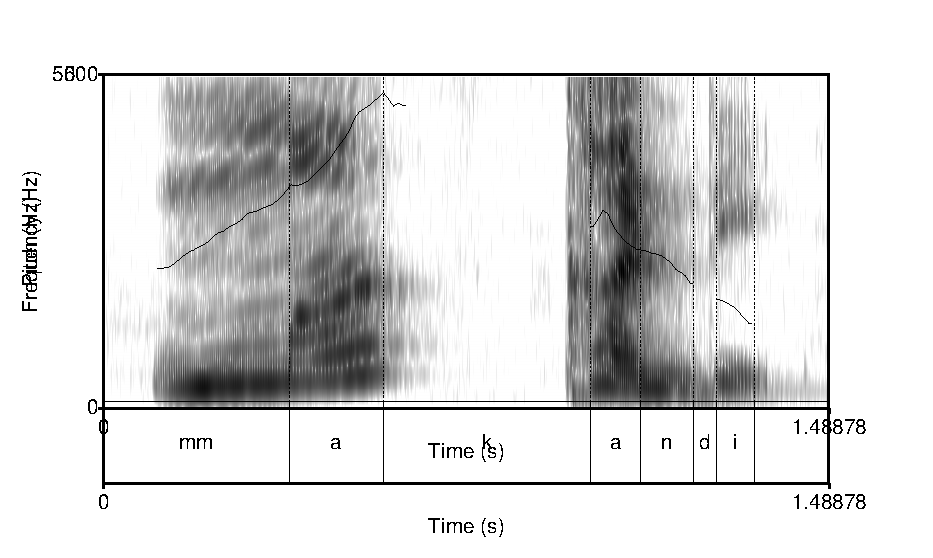
\includegraphics[height=0.3\textheight]{./pics/mmakandi-asp.eps}
 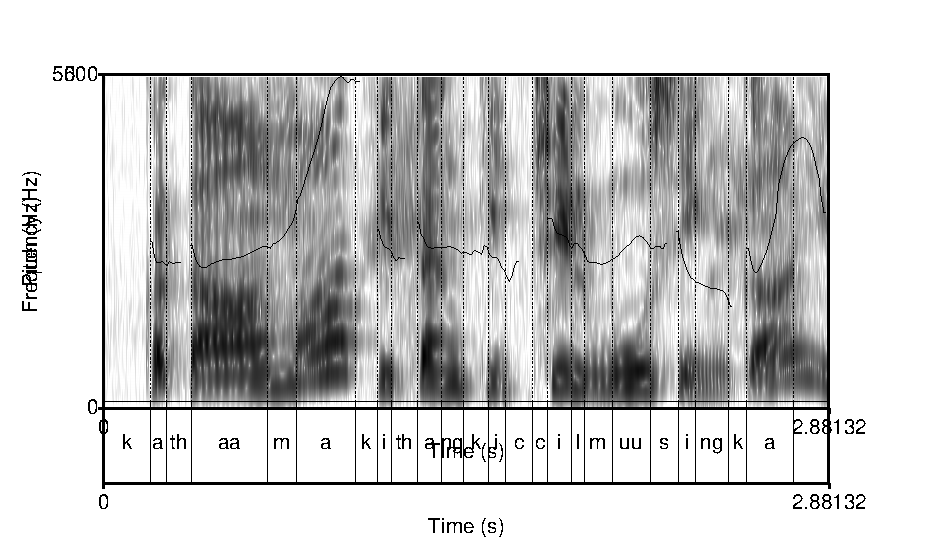
\includegraphics[height=0.3\textheight]{./pics/kathaamakiccilmuusingka.eps}

 \caption{It is rare to find aspirated consonants in SLM, indentified by long VOTs, like the [k] in \phontrs{ka\postalvn\postalvd i}{Kandy (town)} the example above, which has a VOT of 0.049s. One can see from the black shading that the closure is already released, but the voicing has not started yet (indicated by the pitch line).
It is much more common to have VOTs under 0.020s, as is the case with all the stops in the example below}
 \label{fig:phon:vot:mmakang-asp}
\end{figure}

% \paragraph{VOT in intervocalic position}
\begin{figure}
 \centering
 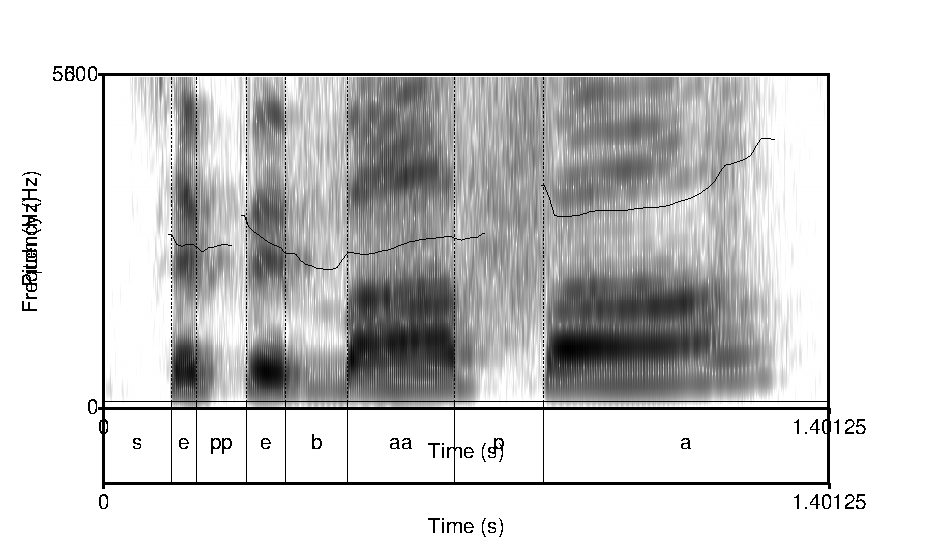
\includegraphics[height=0.3\textheight]{./pics/seppebaapa.eps}
 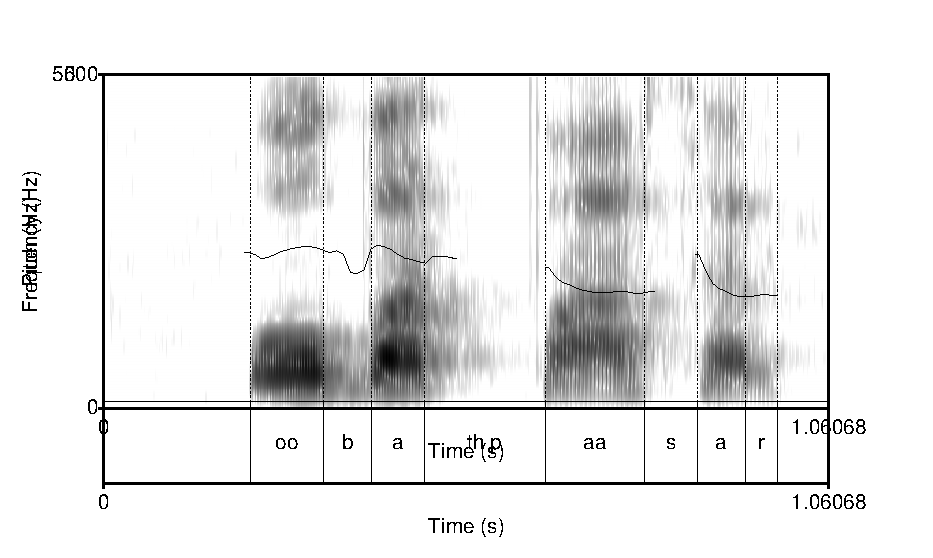
\includegraphics[height=0.3\textheight]{./pics/oobathpaasar.eps}
 \caption{[p] in intervocalic position [a:pa] has a VOT close to zero. [b] in intervocalic position between two morphemes is fully voiced. (above). [b] in morpheme-internal intervocalic position is fully voiced, /p/ in the onset of [pa:sar] has a VOT close to zero (below).}
 \label{fig:phon:vot:oobathpaasar}
\end{figure}

% \paragraph{VOT in intervocalic position, geminated}


\begin{figure}
 \centering
 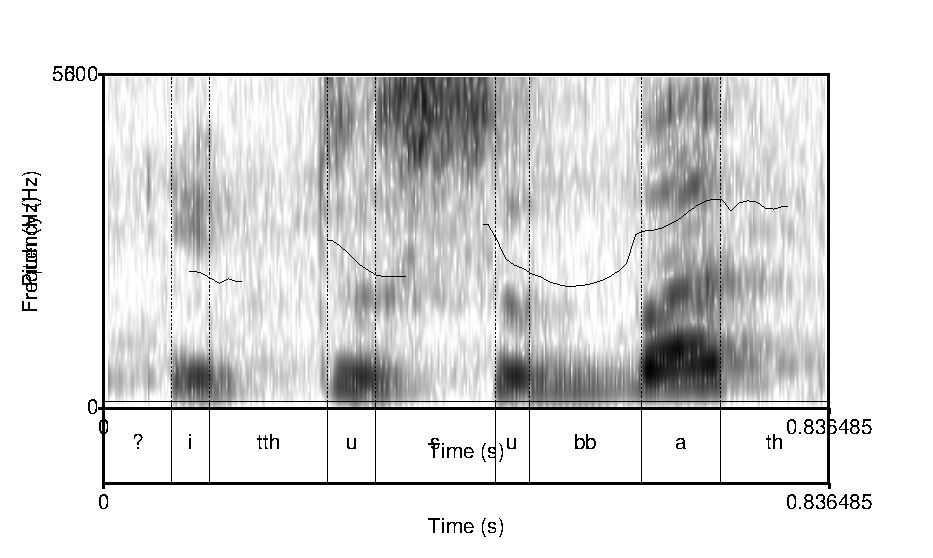
\includegraphics[height=0.3\textheight]{./pics/itthusubbath.eps}
%
 \caption{The  long dental stop in [i\dentt:u] has a VOT close to zero, the  long labial stop in [sub:a\dentt] is fully voiced.}
 \label{fig:phon:vot:itthusubbath}
\end{figure}



% \paragraph{VOT after /s-/}

\begin{figure}
 \centering
 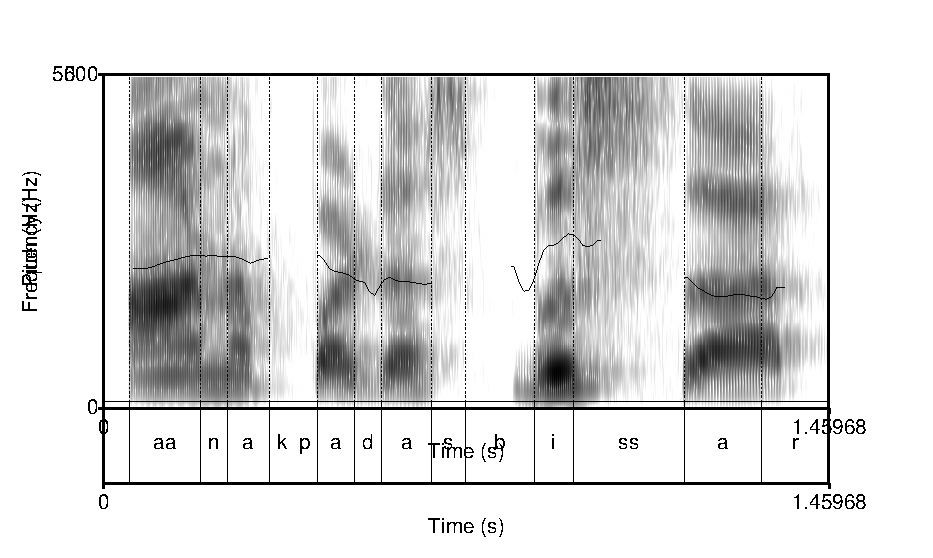
\includegraphics[height=0.3\textheight]{./pics/sbissar.eps}

 \caption{Even after the voiceless fricative [s-], /b/  has a negative VOT of -0.045s. [p] in [pada] has a VOT close to zero.}
 \label{fig:phon:vot:bissar}
\end{figure}


\begin{figure}
 \centering
 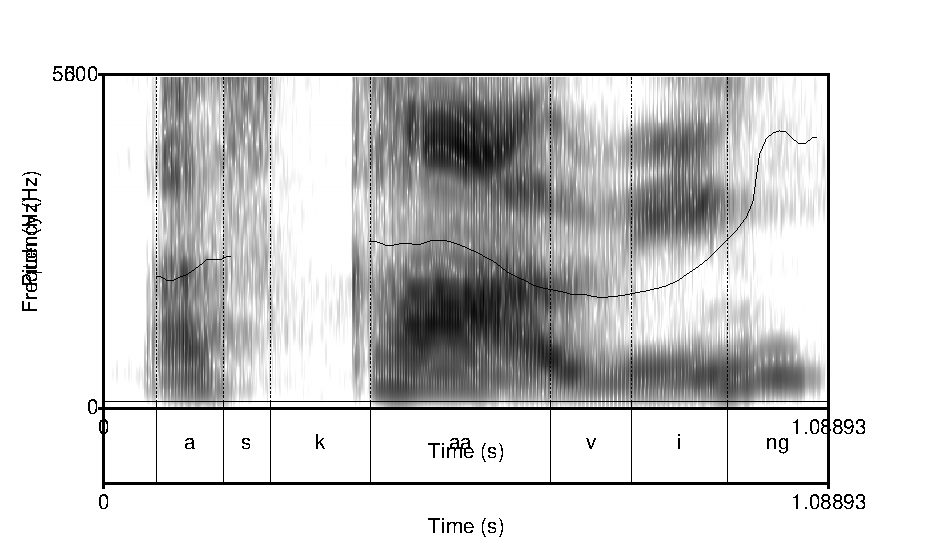
\includegraphics[height=0.3\textheight]{./pics/askaaving.eps}

 \caption{After the voiceless fricative /s/, [k] has a VOT of 0.027s.}
 \label{fig:phon:vot:askaaving}
\end{figure}


\begin{table}
\begin{center}
% use packages: array
\begin{tabular}{lllll}
 & initial & intervocalic & geminated & following s- \\
voiced &  &  &  &  \\ 
voiceless &  &  &  & 
\end{tabular}
\end{center}
\caption{Voice onset times for different environments}
\label{tab:phon:VOT}
\end{table}
